%%%%%%%%%%%%%%%%%%%%%%%%%%%%%%%%%%%%%%%%%%%%%%%%%%%%%%%%%%%%%%%%%%%%%%%%%%%%%%%%%%%%%%%%%%%%%%%%%%%%%%%%%
%%%%%%%%%%%%%%%%%%%%%%%%%%%%%%%%%%%%%%%%%%%% Header %%%%%%%%%%%%%%%%%%%%%%%%%%%%%%%%%%%%%%%%%%%%%%%%%%%%%
%%%%%%%%%%%%%%%%%%%%%%%%%%%%%%%%%%%%%%%%%%%%%%%%%%%%%%%%%%%%%%%%%%%%%%%%%%%%%%%%%%%%%%%%%%%%%%%%%%%%%%%%%

\documentclass[a4paper,titlepage,11pt,twosides,floatssmall]{mwrep}

\usepackage[left=2.5cm,right=2.5cm,top=2.5cm,bottom=2.5cm]{geometry} % Pages' geometry and layout
\usepackage[OT1]{fontenc} % Defines encoding for fonts (OT1 - original TeX encoding) 
\usepackage{polski} % Polish language specifics
\usepackage{amsmath} % Mathematical commands
\usepackage{amsfonts} % Fonts commands
\usepackage{amssymb} % Symbolical commands
\usepackage{graphicx} % Importing external graphics
\usepackage{float} % Forcing plot's position
\usepackage{url} % Web-related text (urls, mail adresses, etc.)
\usepackage{tikz} % Creating graphical elements like lines, dots, curves, figures
\usepackage{rotating} % Rotating objects of an arbitrary angle
\usepackage[percent]{overpic} % Makes it able to put LaTeX commands onto the included graphics (with a dedicated environment)
\usepackage[cp1250]{inputenc} % Non-standrard encoding of the LaTeX files
\usepackage{xcolor} % Easy driver-independent access to several kinds of color tints, shades, tones, and mixes of arbitrary colors
\usepackage{pgfplots} % High-quality function plots in normal or logarithmic scaling with a user-friendly interface
\usepackage{listings} % Source code printer
\usepackage{matlab-prettifier} % Matlab source code printer
\usepackage{enumitem} % List environments
\usepackage{siunitx} % Physical units
\usepackage{subfig} % Subfigures
\usepackage{placeins} % Places figures in sections they were introduced

% tikz packages choice
\usetikzlibrary{arrows,calc,decorations.markings,math,arrows.meta}
\usetikzlibrary{pgfplots.groupplots}

% siunitx settings
\sisetup{detect-weight,exponent-product=\cdot,output-decimal-marker={,},per-mode=symbol,binary-units=true,range-phrase={-},range-units=single}
\SendSettingsToPgf % unifies settings of the pgfplots package with siunitx package

% listings settings
\definecolor{gray}{rgb}{0.95,0.95,0.95}
\lstset{
	backgroundcolor=\color{gray},
	frame=single,
	breaklines=true,
}

% listings styles
\lstdefinestyle{customlatex}{
	basicstyle=\footnotesize\ttfamily,
	% basicstyle=\small\ttfamily,
}
\lstdefinestyle{customc}{
	breaklines=true,
	frame=tb,
	language=C,
	xleftmargin=0pt,
	showstringspaces=false,
	basicstyle=\small\ttfamily,
	keywordstyle=\bfseries\color{green!40!black},
	commentstyle=\itshape\color{purple!40!black},
	identifierstyle=\color{blue},
	stringstyle=\color{orange},
}
\lstdefinestyle{custommatlab}{
	captionpos=t,
	breaklines=true,
	frame=tb,
	xleftmargin=0pt,
	language=matlab,
	showstringspaces=false,
	% basicstyle=\footnotesize\ttfamily,
	basicstyle=\scriptsize\ttfamily,
	keywordstyle=\bfseries\color{green!40!black},
	commentstyle=\itshape\color{purple!40!black},
	identifierstyle=\color{blue},
	stringstyle=\color{orange},
}

% Text field size (without header and footer - bez "�ywej paginy")
\textwidth 160mm \textheight 247mm

% pgfplots settings
\pgfplotsset{
	tick label style={font=\scriptsize},
	label style={font=\small},
	legend style={font=\small},
	title style={font=\small}
}

\def\figurename{Rys.}
\def\tablename{Tab.}

% Max number of floating elements configuration
\setcounter{topnumber}{0} % default : 2
\setcounter{bottomnumber}{3} % default : 1
\setcounter{totalnumber}{5} % default : 3

\renewcommand{\textfraction}{0.01} % default : 0.2
\renewcommand{\topfraction}{0.95} % default : 0.7
\renewcommand{\bottomfraction}{0.95} % default : 0.3
\renewcommand{\floatpagefraction}{0.35} % default : 0.5

% Path to the graphics
\graphicspath{ {./img/} }

%%%%%%%%%%%%%%%%%%%%%%%%%%%%%%%%%%%%%%%%%%%%%%%%%%%%%%%%%%%%%%%%%%%%%%%%%%%%%%%%%%%%%%%%%%%%%%%%%%%%%%%%%
%%%%%%%%%%%%%%%%%%%%%%%%%%%%%%%%%%%%%% Document utilities %%%%%%%%%%%%%%%%%%%%%%%%%%%%%%%%%%%%%%%%%%%%%%%
%%%%%%%%%%%%%%%%%%%%%%%%%%%%%%%%%%%%%%%%%%%%%%%%%%%%%%%%%%%%%%%%%%%%%%%%%%%%%%%%%%%%%%%%%%%%%%%%%%%%%%%%%

% Title Page Data
\title{\bf Sprawozdanie z~laboratorium nr 4\vskip 0.1cm}
\author{Pawe� Bugyi, Marcin Michalski, Krzysztof Pierczyk}
\date{2020}

% Maketitle macro
\makeatletter
\renewcommand{\maketitle}
{
	\begin{titlepage}
		\begin{center}{
			\LARGE {\bf
			Wydzia� Elektroniki i Technik Informacyjnych}}\\
			\vspace{0.4cm}
			{\LARGE {\bf Politechnika Warszawska}}\\
			\vspace{0.3cm}
		\end{center}
		\vspace{5cm}
		\begin{center}
			{\bf \LARGE Projektowanie uk�ad�w sterowania\\ (projekt grupowy) \vskip 0.1cm}
		\end{center}
		\vspace{1cm}
		\begin{center}
			{\bf \LARGE \@title}
		\end{center}
		\vspace{2cm}
		\begin{center}
			{\bf \Large \@author \par}
		\end{center}
		\vspace*{\stretch{6}}
		\begin{center}
			\bf{\large{Warszawa, \@date\vskip 0.1cm}}
		\end{center}
	\end{titlepage}
}
\makeatother

%%%%%%%%%%%%%%%%%%%%%%%%%%%%%%%%%%%%%%%%%%%%%%%%%%%%%%%%%%%%%%%%%%%%%%%%%%%%%%%%%%%%%%%%%%%%%%%%%%%%%%%%%
%%%%%%%%%%%%%%%%%%%%%%%%%%%%%%%%%%%%%%%%%%% Document %%%%%%%%%%%%%%%%%%%%%%%%%%%%%%%%%%%%%%%%%%%%%%%%%%%%
%%%%%%%%%%%%%%%%%%%%%%%%%%%%%%%%%%%%%%%%%%%%%%%%%%%%%%%%%%%%%%%%%%%%%%%%%%%%%%%%%%%%%%%%%%%%%%%%%%%%%%%%%

\begin{document}

% Pages' style formatting
\frenchspacing
\pagestyle{uheadings}

% Use maketitle macro to build title page
\maketitle

% Insert parts of the report
\tableofcontents
\chapter{Wst�p}
Drugi projekt z~Projektowania Uk�ad�w Sterowania (PUST) stanowi� rozszerzenie projektu pierwszego. Ponownie zaj�li�my si� badaniem obiektu, danego funkcj� napisan� w Matlabie oraz projektowaniem i strojeniem do niego uk�adu regulacji. Rozszerzenie polega�o na przej�ciu z~obiektu typu SISO (\textit{ang.} Single-input-single-output) na obiekt typu MISO (\textit{ang.} Multiple-input-\\single-output), w~kt�rym jedno z wej�� by�o wej�ciem niesterowanym (zak��ceniem procesu). Modyfikacja ta pozwoli�a nam na zweryfikowanie efektywno�ci algorytmu regulacji predykcjynej DMC ((\textit{ang.} Dynamic Matrix Control) przystosowanego do pracy z mierzalnym zak��ceniem. Niniejsze sprawozdanie stanowi podsumowanie ca�ego naszego trudu, wszystkich wylanych �ez, nieprzespanych nocy oraz pobitych element�w zastawy domowej zwi�zanych z realizacj� projektu.
\chapter{Badanie poprawno�ci punktu pracy}

Pierwsze zadanie sprowadza�o si� do zweryfikowania poprawno�ci, podanego w~tre�ci zadania, punktu pracy $U_{pp}=\num{1.7}$, $Y_{pp}=\num{2}$. Weryfikacja polega�a na podaniu na wej�cie obiektu sta�ej warto�ci pobudzenia $U=\num{1.7}$ przy jednoczesnym za�o�eniu, �e warto�� wyj�cia w~przesz�o�ci ustalona by�a na poziomie $Y=\num{2.0}$ i sprawdzeniu, czy warto�� ta ulegnie zmianie. Wynik eksperymentu zosta� przedstawiony na rys. \ref{work_point_check}. Zgodnie z~danymi podanymi w~tre�ci zadania, punkt $U=\num{1.7},Y=\num{2}$ jest rzeczywi�cie punktem pracy.

\vskip 0.5cm
\begin{figure}[h]
    \centering
        \begin{tikzpicture}
            \begin{axis}[
                    width=0.5\textwidth,
                    xmin=0,xmax=100,ymin=0,ymax=3,
                    xlabel={$t [s]$},
                    ylabel={$y(t)$},
                    xtick={0, 25, 50, 75, 100},
                    ytick={0,0.5,1.0,1.5, 2.0, 2.5, 3.0},
                    legend pos=south east,
                    y tick label style={/pgf/number format/1000 sep={,}},
                ]
                \addplot[const plot, blue]                file {data/exercise_1/work_point_check.txt};
                \legend{$y(t)$}
            \end{axis}
        \end{tikzpicture}
    \caption{Przebieg warto�ci wyj�ciowej procesu po podaniu sta�ego wej�cia $U=\num{1.7}$}
    \label{work_point_check}
\end{figure}
\vskip 0.5cm

\chapter{Wyznaczanie odpowiedzi skokowej}

Drugie zadanie polega�o na wyznaczeniu odpowiedzi uk�adu na kilka skokowych zmian warto�ci sygna�u steruj�cego przy zachowaniu ogranicze� ich warto�ci. Sygna� steruj�cy musi zawiera� si� w~przedziale $U\in[\num{1.4}; \num{2.0}]$. �rodkowi tego przedzia�u odpowiada punkt pracy uk�adu weryfikowany w~zadaniu nr 1, kt�ry w~tym przypadku pos�u�y� jako warto�� startowa. Obiekt zosta� doprowadzony do punktu pracy poprzez zainicjalizowanie wektor�w warto�ci steruj�cej i~warto�ci wyj�ciowej odpowiednimi warto�ciami $U=\num{1.7},Y=\num{2}$, co zosta�o przedstawione na poni�szym listingu.

\vskip 0.5cm
\begin{lstlisting}[style=Matlab-editor]
    U_init = ones(STEPS_NUM,1) * 1.7;
    Y_init = ones(STEPS_NUM,1) * 2;
\end{lstlisting} 
\vskip 0.5cm

Wykonano ��cznie 8 skok�w warto�ci steruj�cej, przy czym cztery z~nich mia�y warto�ci ujemne, a~cztery warto�ci dodatnie. Wszystkie zosta�y r�wno rozmieszczone pomi�dzy punktem pocz�tkowym, a~minimaln�/maksymaln� dozwolon� warto�ci�. Wyniki pomiar�w przedstawiono na rys. \ref{step_responses}. Dane pomiarowe zosta�y przesuni�te w~czasie tak, aby punkt pocz�tkowy ($Czas=0s$) by� momentem wykonania skoku sterowania.

\vskip 1cm
\begin{figure}[h]
    \centering
        \begin{tikzpicture}
            \begin{axis}[
                    width=0.5\textwidth,
                    xmin=0,xmax=100,ymin=1.5,ymax=2.5,
                    xlabel={$t [s]$},
                    ylabel={$y(t)$},
                    xtick={0,25,50,75,100},
                    ytick={1.5, 1.6, 1.7, 1.8, 1.9, 2.0, 2.1, 2.2, 2.3, 2.4, 2.5},
                    legend pos=south east,
                    legend style={font=\tiny},
                    y tick label style={/pgf/number format/1000 sep={,}},
                ]
                
                \addplot[const plot, blue]               file {data/exercise_2/step_response_1.txt};
                \addplot[const plot, cyan]               file {data/exercise_2/step_response_2.txt};
                \addplot[const plot, green]              file {data/exercise_2/step_response_3.txt};
                \addplot[const plot, lime]               file {data/exercise_2/step_response_4.txt};
                \addplot[const plot, olive]              file {data/exercise_2/step_response_5.txt};
                \addplot[const plot, yellow]             file {data/exercise_2/step_response_6.txt};
                \addplot[const plot, orange]             file {data/exercise_2/step_response_7.txt};
                \addplot[const plot, red]                file {data/exercise_2/step_response_8.txt};

                \legend{$\Delta U=\num{0.3}$,$\Delta U=\num{0.225}$,$\Delta U=\num{0.150}$,$\Delta U=\num{0.075}$,$\Delta U=\num{-0.075}$,$\Delta U=\num{-0.150}$,$\Delta U=\num{-0.225}$,$\Delta U=\num{-0.3}$}

            \end{axis}
        \end{tikzpicture}
    \caption{Przebieg warto�ci wyj�ciowej procesu przy skokowej zmianie sygna�u steruj�cego}
    \label{step_responses}
\end{figure}
\vskip 1cm

Druga cz�� zadania polega�a na zbadaniu charakterystyki statycznej uk�adu i~okre�leniu, czy proces jest w przybli�eniu liniowy. Zebrawszy odpowiedzi skokowe stworzyli�my wektor par $(U_{pp}, Y_{pp})$ reprezentuj�cych punkty pracy uk�adu. Punkty te wyrysowane na p�aszczy�nie ukaza�y charakterystyk�, kt�r� mo�emy obserwowa� na rys. \ref{static_characteristic}

\vskip 0.5cm
\begin{figure}[H]
    \centering
        \begin{tikzpicture}
            \begin{axis}[
                    width=0.5\textwidth,
                    xmin=1.4,xmax=2,ymin=1.5,ymax=2.5,
                    xlabel={$u$},
                    ylabel={$y(u)$},
                    xtick={1.4,1.5,1.6, 1.7, 1.8, 1.9, 2.0},
                    ytick={1.5, 1.6, 1.7, 1.8, 1.9, 2.0, 2.1, 2.2, 2.3, 2.4, 2.5},
                    legend pos=south east,
                    x tick label style={/pgf/number format/1000 sep={,}},
                    y tick label style={/pgf/number format/1000 sep={,}},
                ]
                \addplot[blue]                file {data/exercise_2/static_characteristic.txt};
            \end{axis}
        \end{tikzpicture}
    \caption{Charakterystyka statyczna obiektu}
    \label{static_characteristic}
\end{figure}
\vskip 0.5cm

Jak wida�, obiekt wykazuje silnie liniowy charakter. Pozwala to wyznaczy� wzmocnienie statyczne uk�adu, czyli warto�� zmiany wyj�cia uk�adu przy jednostkowej zmianie warto�ci sygna�u steruj�cego. Obliczaj�c stosunek zmiany na wyj�ciu uk�adu do zmiany warto�ci steruj�cej przy skoku z~$U=\num{1.7}$ do $U=\num{2.0}$ otrzymujemy r�wnanie pokazane na rys. \ref{static_gain}.

\vskip 0.5cm
\begin{equation}
    K = \dfrac{\Delta Y}{\Delta U} = \dfrac{\num{2.4320}}{\num{0.3}} = \num{0.6945}
    \label{static_gain}
\end{equation}
\vskip 0.5cm

\chapter{Wyznaczanie odpowiedzi skokowej do DMC}
Kolejnym krokiem do realizacji projektu by�o opracowanie wynik�w, otrzymanych w zadaniu drugim, i~uzyskanie z~nich odpowiedzi skokowej w~postaci wykorzystywanej w~algorytmie DMC. Bior�c pod uwag� wniosek dotycz�cy liniowo�ci obiektu w~ca�ym badanym zakresie, do tego celu wybra� mogli�my dowolne odpowiedzi skokowe z obu tor�w. Zdecydowali�my si� na skoki z~$u = 0$ do $u = 1$ oraz z~$z = 0$ do $z = 1$. Warto�� wej�ciowa toru komplementarnego by�a zerowa w~przypadku obydwu skok�w. Odpowiedzi te zosta�y przedstawione na rysunkach \ref{u_step_response} i \ref{z_step_response}.

\begin{figure}[h]
\centering
\begin{tikzpicture}
\begin{axis}[
width=0.5\textwidth,
xmin=0,xmax=190,ymin=0,ymax=3,
xlabel={$k$},
ylabel={$y(k)$},
legend pos=south east,
y tick label style={/pgf/number format/1000 sep=},
]
\addplot[red , semithick ] file { data/exercise_3/U_step_response_DMC.txt};
\legend{y(k)}
\end{axis}
\end{tikzpicture}
\caption{Odpowied� skokowa DMC na sygna� steruj�cy}
\label{u_step_response}
\end{figure}

\begin{figure}[h]
\centering
\begin{tikzpicture}
\begin{axis}[
width=0.5\textwidth,
xmin=0,xmax=40,ymin=0,ymax=2,
xlabel={$k$},
ylabel={$y(k)$},
legend pos=south east,
y tick label style={/pgf/number format/1000 sep=},
]
\addplot[red , semithick ] file { data/exercise_3/Z_step_response_DMC.txt};
\legend{y(k)}
\end{axis}
\end{tikzpicture}
\caption{Odpowied� skokowa DMC na zak��cenie}
\label{z_step_response}
\end{figure}

Liniowo�� obiektu i~brak ogranicze� warto�ci sygna��w pozwoli�y nam wybra� dogodne warto�ci skok�w co zniwelowa�o potrzeb� przeskalowywania otrzymanej odpowiedzi. Jedynym zabiegiem, jaki musieli�my wykona�, by�o wybranie z wektor�w pr�bek odpowiedzi tych, o~w�a�ciwych indeksach. Jako �e skoki odbywa�y si� w~chwili $n = 0$, do odpowiedzi skokowej zosta�y wzi�te tylko pr�bki z~chwil $n >= 1$. Wst�pne horyzonty dynamiki zosta�y wybrane tak, aby zmiana warto�ci wyj�cia w~chwilach $n > D$, gdzie $D$ to wybrany horyzont, by�y niewi�ksze ni� \num{0.01}\% warto�ci maksymalnej.

\section{Panel HMI i~kontrola trajektorii zadanej}

\vskip 0.5cm
\begin{figure}[H]
    \centering
    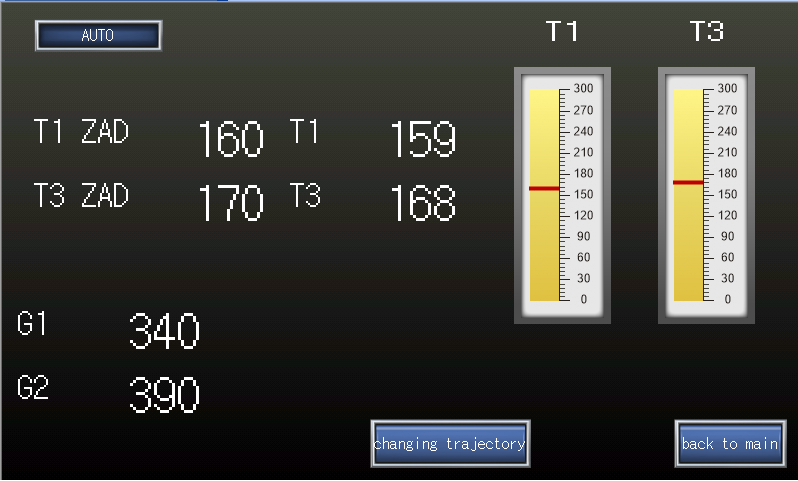
\includegraphics[scale=0.7]{HC_Main.png}
    \caption{Cz�� g��wna panelu operatora}
    \label{hc_main}
\end{figure}
\vskip 0.5cm

Stworzony panel operatorski posiada trzy poziomy. Pierwszy z~nich pozwala po prostu na wyb�r obiektu sterowania. Po wej�ciu w~sekcj� po�wi�conom stanowisku grzej�co-ch�odz�cemu ukazuje nam si� obraz widoczny na rys. \ref{hc_main}. Warto�ci temperatur $T1$ i~$T3$ zosta�y zwizualizowane w~postaci s�upk�w z~podzia�k� i~poruszaj�cych si� po nich czerwonych poprzeczkach. Dok�adna warto�� liczbowa wy�wietlana jest na lewo od wska�nik�w. Na tej samej wysoko�ci, po lewej stronie panelu znajduj� si� pola pozwalaj�ce ustawi� warto�� zadan� \footnote{W~przypadku sterowania automatycznego}. Powy�ej zosta� z~kolei umiejscowiony przycisk, kt�ry umo�liwia prze��czanie regulatora mi�dzy trybem manualnym a~automatycznym. W~przypadku pierwszego z~nich warto�ci sterowa� mog� zosta� ustawione przy pomocy p�l w~lewej dolnej cz�ci ekranu.

Po naci�ni�ci�ciu przycisku "changing trajectory" u�ytkownik przechodzi do panelu, w~kt�rym mo�liwe jest ustawienie zmienianej skokowo trajektorii zadanej (rys. \ref{hc_trajectory}). Trajektoria sk�ada si� z~pi�ciu przedzia��w czasowych, ka�dy o~d�ugo�ci r�wnej warto�ci ustawionej w~polu "duration". Dla ka�dego z przedzia��w mo�liwe jest ustawienie innej warto�ci zadanej. Po zako�czeniu ostatniego segmentu trajektoria warto�ci zadanej jest zap�tlana. Po ustawieniu porz�danej trajektorii u�ytkownik mo�e uruchomi� jej realizacj� poprzez prze��czenie przycisku w~lewym g�rnym rogu ekranu. Implementacja ta rozwi�zuje problem postawiony w~zadaniu 5. Realizacja programowa odbywa si� poprzez prost� sekwencj� instrukcji warunkowych widocznych na poni�szym listingu. Wykonywana jest ona przy ka�dej iteracji programu.

\vskip 1cm
\begin{lstlisting}[style=customc,frame=single] 
	IF HC_TRAJ_ON THEN
		IF traj = 0 THEN
			HC_DMC.HC_T1_ZAD := HC_T1_TRAJ1;
			HC_DMC.HC_T2_ZAD := HC_T2_TRAJ1;
		ELSIF traj = 1*HC_DURATION THEN
			HC_DMC.HC_T1_ZAD := HC_T1_TRAJ2;
			HC_DMC.HC_T2_ZAD := HC_T2_TRAJ2;
		ELSIF traj = 2*HC_DURATION THEN
			HC_DMC.HC_T1_ZAD := HC_T1_TRAJ3;
			HC_DMC.HC_T2_ZAD := HC_T2_TRAJ3;
		ELSIF traj = 3*HC_DURATION THEN
			HC_DMC.HC_T1_ZAD := HC_T1_TRAJ4;
			HC_DMC.HC_T2_ZAD := HC_T2_TRAJ4;
		ELSIF traj = 4*HC_DURATION THEN
			HC_DMC.HC_T1_ZAD := HC_T1_TRAJ5;
			HC_DMC.HC_T2_ZAD := HC_T2_TRAJ5;
		ELSIF traj = 5*HC_DURATION THEN
			traj :=0;
		ELSE;
		END_IF;
		traj := traj + 1;
	END_IF;
\end{lstlisting}
\vskip 1cm

\vskip 0.5cm
\begin{figure}[H]
    \centering
    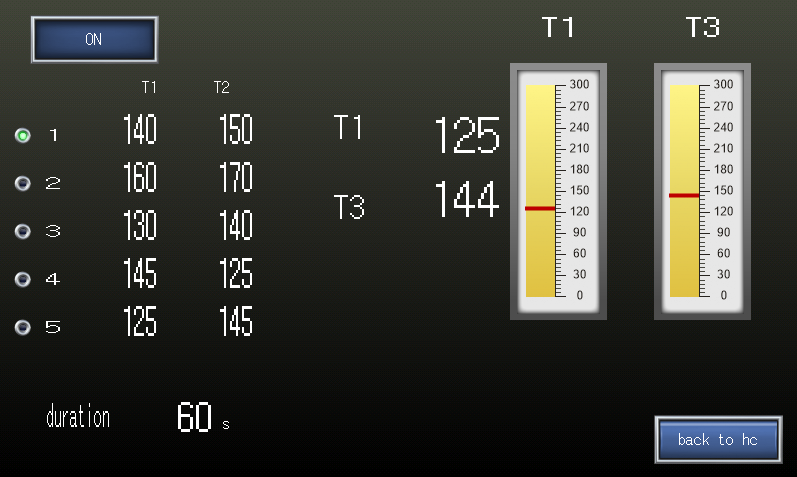
\includegraphics[scale=0.7]{HC_trajectory.png}
    \caption{Panel umo�liwiaj�cy konfiguracj� trajektorii zadanej dla stanowiska G-C}
    \label{hc_trajectory}
\end{figure}
\vskip 0.5cm
\chapter{Wp�yw zak��cenia sinusoidalnego na prac� algorytmu DMC}
W tym zadaniu wykorzystujemy algorytm DMC z zadania 5. Zak��cenie ma posta� sinusoidy danej wzorem:
\begin{equation}
Z(k) = Amplitude * sin(2\pi* freq / (0.5 * k) )
\end{equation}
gdzie k to numer pr�bki. 
Z(k) oznacza wektor zawieraj�cy przebieg sygna�u zak��caj�cego.
\newpage

\begin{center}
\begin{figure}[H]
\makebox[\textwidth]{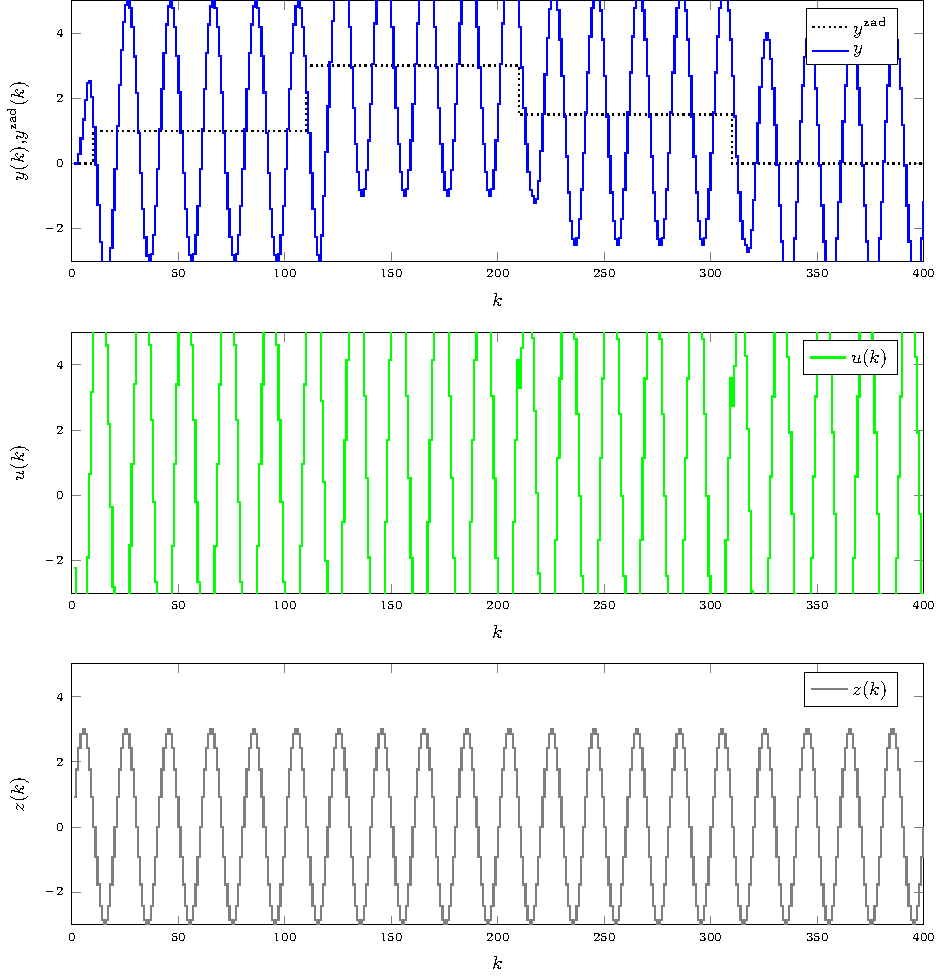
\includegraphics[width=\paperwidth]{data/exercise_6/Desired_output_plot_iter_01_ampl_3_freq_0.1_Dz_20_error_3205.4653.pdf}}
\caption{amplitude=3, freq=0.1, Dz=20, error=3205.4653}
\label{Desired_output_plot_iter_01_ampl_3_freq_0.1_Dz_20_error_3205.4653}
\end{figure}
\end{center}
\begin{center}
\begin{figure}[H]
\makebox[\textwidth]{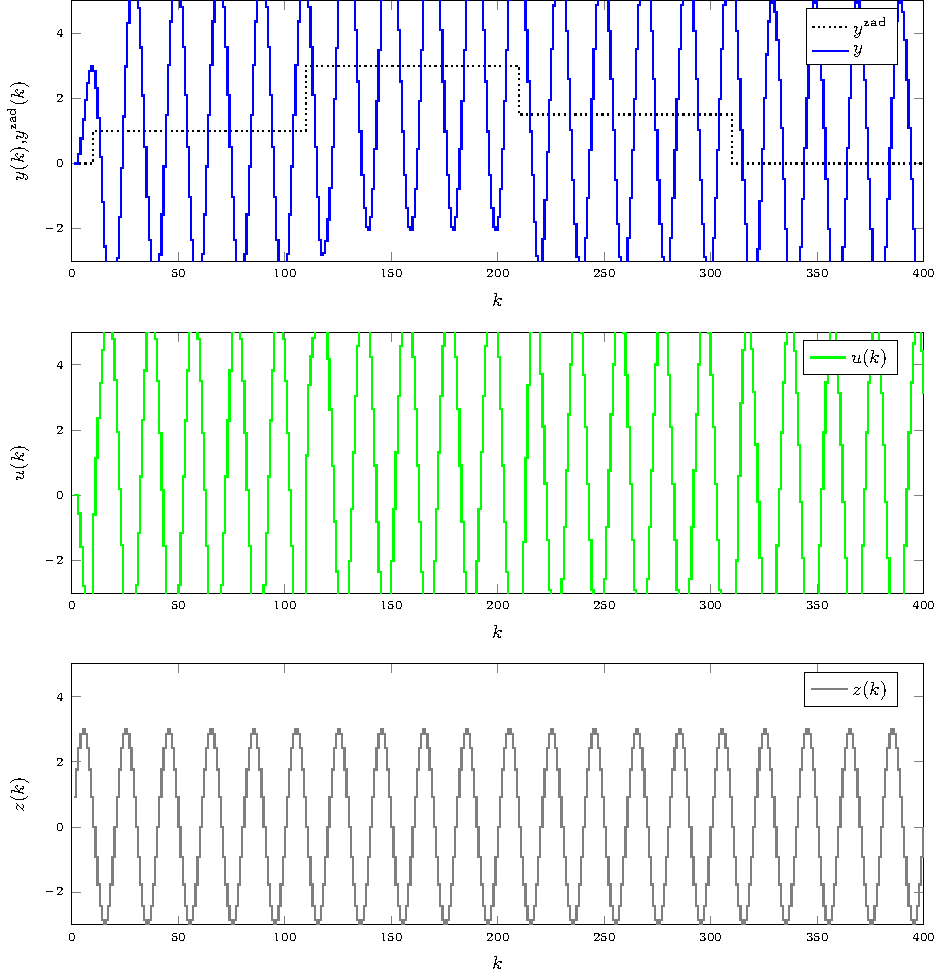
\includegraphics[width=\paperwidth]{data/exercise_6/Desired_output_plot_iter_02_ampl_3_freq_0.1_Dz_0_error_5112.5582.pdf}}
\caption{amplitude=3, freq=0.1, Dz=0, error=5112.5582}
\label{Desired_output_plot_iter_02_ampl_3_freq_0.1_Dz_0_error_5112.5582}
\end{figure}
\end{center}
\begin{center}
\begin{figure}[H]
\makebox[\textwidth]{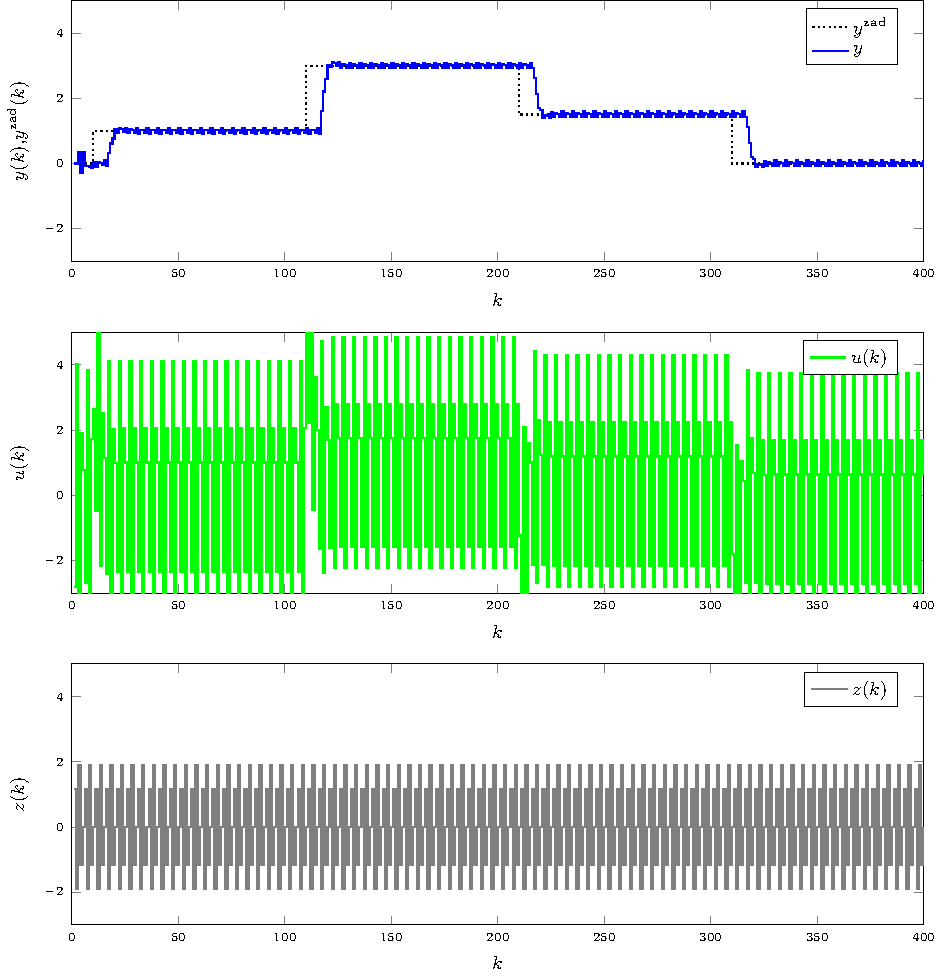
\includegraphics[width=\paperwidth]{data/exercise_6/Desired_output_plot_iter_03_ampl_2_freq_0.8_Dz_20_error_75.3829.pdf}}
\caption{amplitude=2, freq=0.8, Dz=20, error=75.3829}
\label{Desired_output_plot_iter_03_ampl_2_freq_0.8_Dz_20_error_75.3829}
\end{figure}
\end{center}
\begin{center}
\begin{figure}[H]
\makebox[\textwidth]{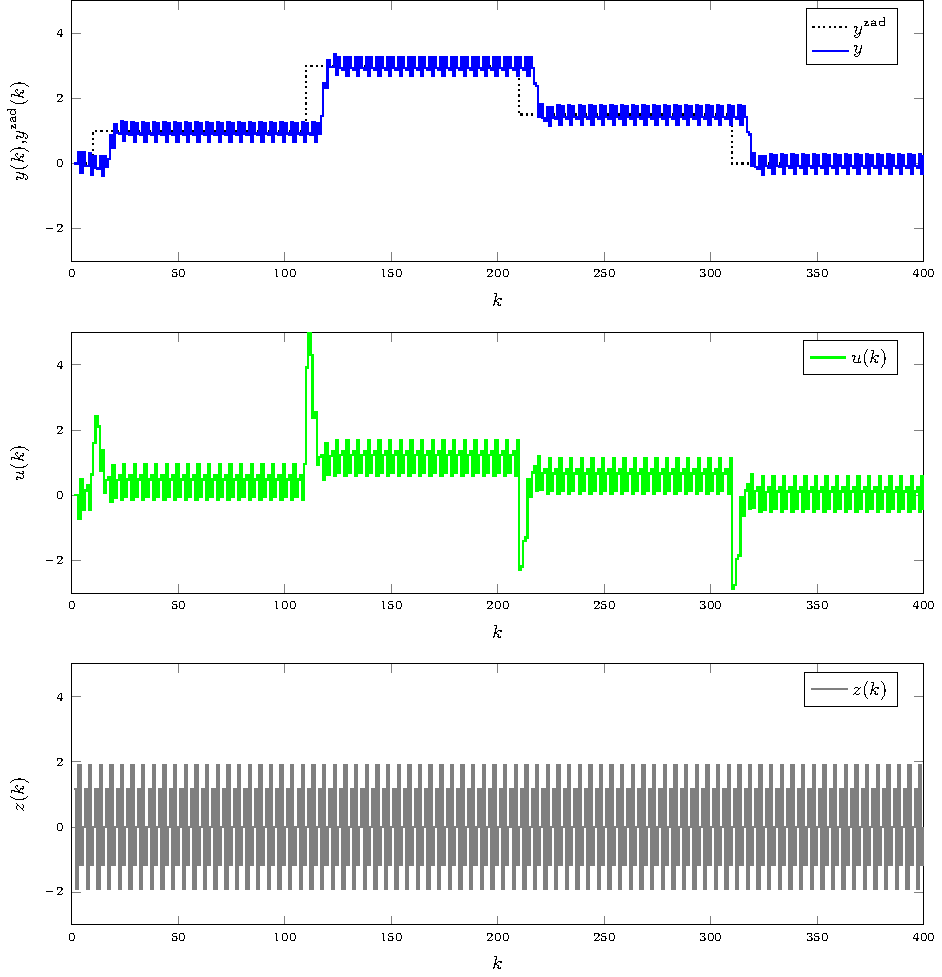
\includegraphics[width=\paperwidth]{data/exercise_6/Desired_output_plot_iter_04_ampl_2_freq_0.8_Dz_0_error_95.3365.pdf}}
\caption{amplitude=2, freq=0.8, Dz=0, error=95.3365}
\label{Desired_output_plot_iter_04_ampl_2_freq_0.8_Dz_0_error_95.3365}
\end{figure}
\end{center}
\begin{center}
\begin{figure}[H]
\makebox[\textwidth]{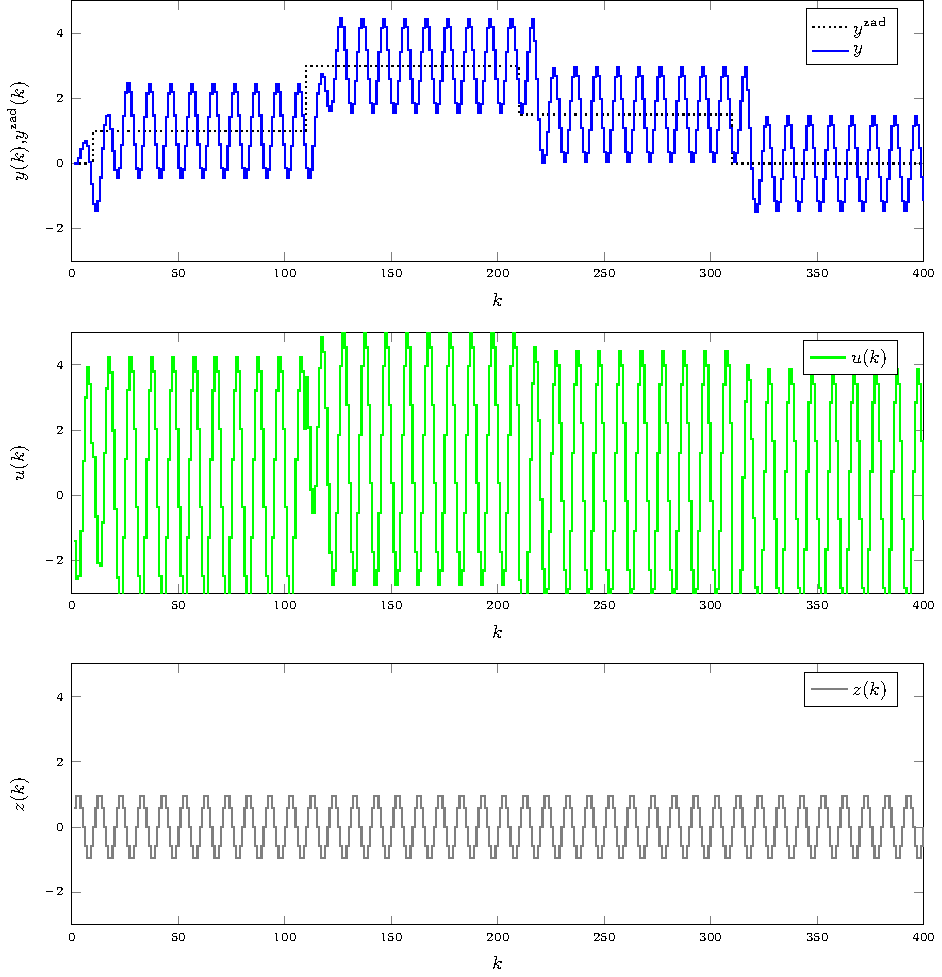
\includegraphics[width=\paperwidth]{data/exercise_6/Desired_output_plot_iter_05_ampl_1_freq_0.2_Dz_20_error_481.7742.pdf}}
\caption{amplitude=1, freq=0.2, Dz=20, error=481.7742}
\label{Desired_output_plot_iter_05_ampl_1_freq_0.2_Dz_20_error_481.7742}
\end{figure}
\end{center}
\begin{center}
\begin{figure}[H]
\makebox[\textwidth]{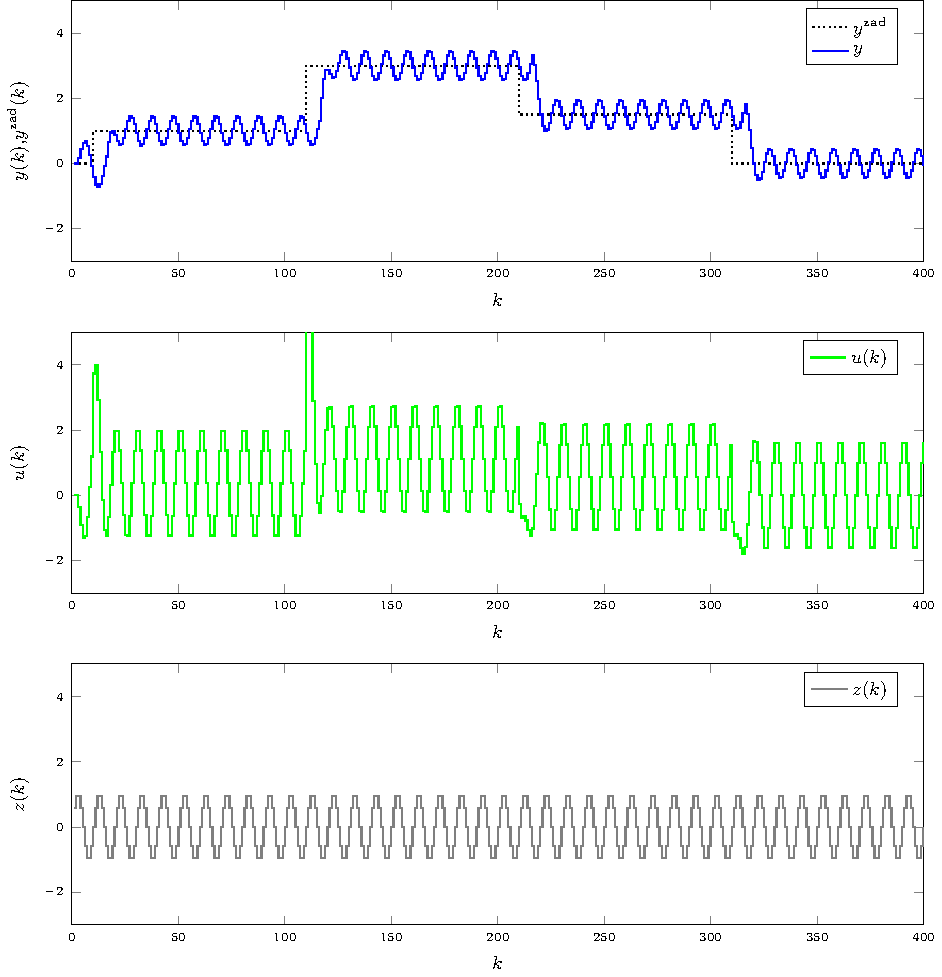
\includegraphics[width=\paperwidth]{data/exercise_6/Desired_output_plot_iter_06_ampl_1_freq_0.2_Dz_0_error_119.0913.pdf}}
\caption{amplitude=1, freq=0.2, Dz=0, error=119.0913}
\label{Desired_output_plot_iter_06_ampl_1_freq_0.2_Dz_0_error_119.0913}
\end{figure}
\end{center}
\begin{center}
\begin{figure}[H]
\makebox[\textwidth]{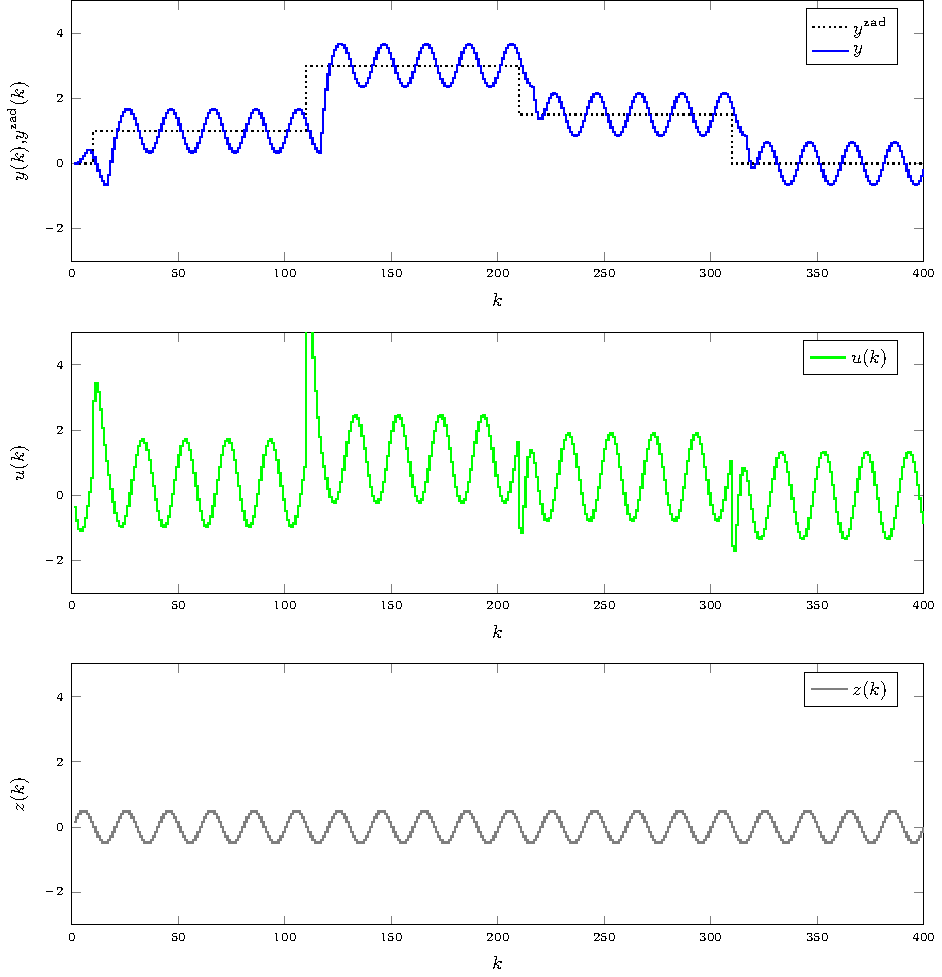
\includegraphics[width=\paperwidth]{data/exercise_6/Desired_output_plot_iter_07_ampl_0.5_freq_0.1_Dz_20_error_160.3299.pdf}}
\caption{amplitude=0.5, freq=0.1, Dz=20, error=160.3299}
\label{Desired_output_plot_iter_07_ampl_0.5_freq_0.1_Dz_20_error_160.3299}
\end{figure}
\end{center}
\begin{center}
\begin{figure}[H]
\makebox[\textwidth]{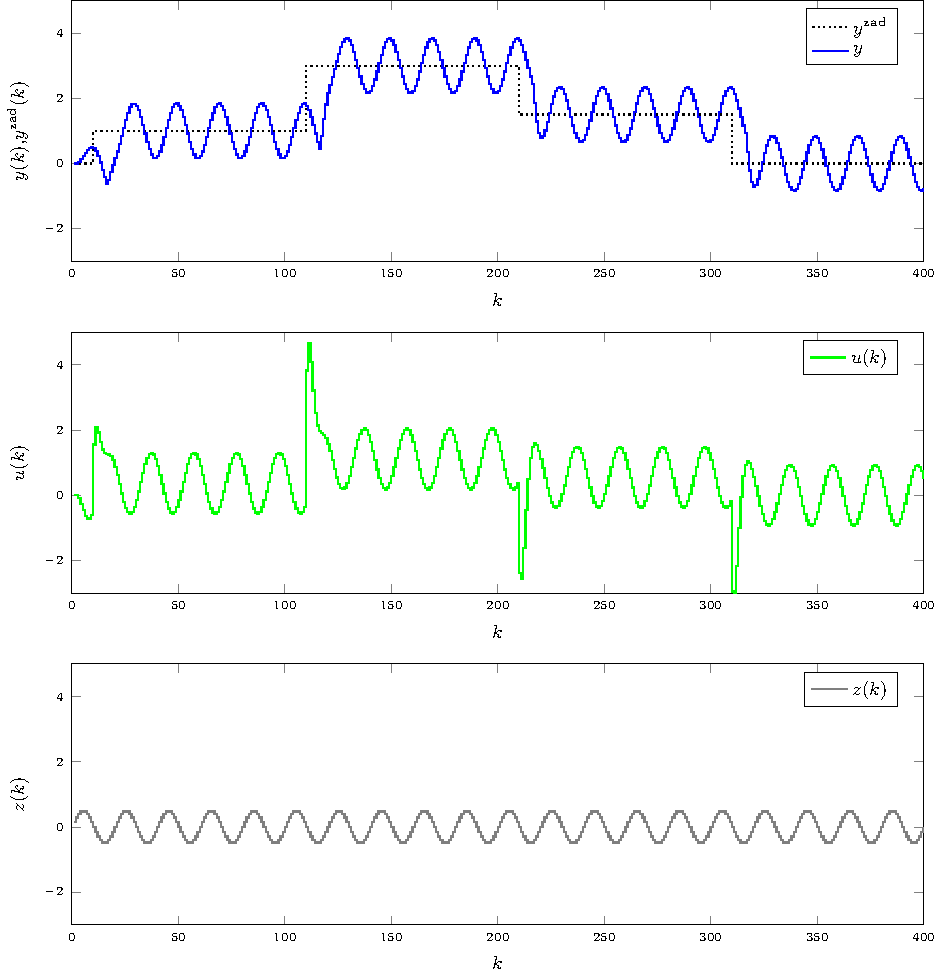
\includegraphics[width=\paperwidth]{data/exercise_6/Desired_output_plot_iter_08_ampl_0.5_freq_0.1_Dz_0_error_215.3014.pdf}}
\caption{amplitude=0.5, freq=0.1, Dz=0, error=215.3014}
\label{Desired_output_plot_iter_08_ampl_0.5_freq_0.1_Dz_0_error_215.3014}
\end{figure}
\end{center}

Jak mo�na zauwa�y�, r�nica w jako�ci regulacji na podstawie przebieg�w z i bez uwzgl�dniania sygna�u zak��caj�cego przez algorytm DMC przy obliczaniu sygna�u steruj�cego jest znacz�ca i tym wi�ksza, czym wy�sza jest amplituda sinusoidy zak��caj�cej.
\section{Charakterystyka statyczna}

Na pierwszy rzut oka stanowisko Inteco mo�na uzna� za obiekt $3 \times 3$. Chwila refleksji uzmys�awia jednak, �e nie wszystkie wej�cia maj� wp�yw na wszystkie wyj�cia. Na przyk�ad rozszczelnienie zaworu poni�ej zbiornika dolnego nie wp�ywa na poziom wody w~zbiorniku g�rnym. Zadanie 7 postawi�o przed nami problem zbadania charakterystyki statycznej obiektu. W~przypadku og�lnego obiektu $3 \times 3$ by�oby to niebagatelne zadania. Wymaga�o by ono najpewniej zbadania stan�w ustalonych wyj�� w~pewnym sze�cianie z~przestrzeni stan�w ustalonych sygna��w wej�ciowych. Dla kraw�dzi takiego sze�cianu ekstrapolowanej z~$n$ punkt�w ($n$ pomiar�w) oznacza�oby to konieczno�� wykonania $n^3$ ekperyment�w! Innym podej�ciem, przy za�o�eniu, �e obiekt jest, przynajmniej w~przybli�eniu, liniowy by�oby zebranie odpowiedzi skokowych dla ka�dego toru wej�cia-wyj�cia i~identyfikacja na ich podstawie macierzy transmitancji obiektu. Z~macierzy tej mo�naby z~kolei w~spos�b analityczny wyznaczy� charakterystyk� statyczn�.


Problem ten mo�na jednak w~znakomitym stopniu upro�ci�, je�eli we�mie si� pod uwag� pewne charakterystyczne cechy obiektu. Za��my, �e obiekt znajduje si� w~stanie ustalonym \footnote{Tak jak w~tre�ci zadania zak�adamy, �e dop�yw do g�rnego zbiornika jest sta�y, �~manipulujemy jeydnie stopniem rozszczelnienia zawor�w}. Je�eli zmienimy stopie� otwarcia zaworu pod zbiornikiem g�rnym, to poziom wody zmieni si� oczywi�cie chwilowo we wszystkich zbiornikach \footnote{Ze zbiornika g�rnego zacznie wyp�ywa� wi�cej wody, zatem wi�cej wody wpadna� b�dzie do zbiornika �rodkowego, przez co zwi�kszy si� w~nim ci�nienie hydrostatyczne. Poskutkuje to zmian� wyp�ywu z~tego zbiornika i~zaj�ciem podobych zmian w~zbiorniku dolnym.}. Zauwa�my jednak, �e po pewnym czasie poziom wody w~zbiorniku g�rnym ustali si� na pewnym poziomie. Je�eli poziom b�dzie utrzymywany, a~dop�yw do zbiornika g�rnego sta�y to b�dzie to znaczy�, �e wy�ywa z niego ta sama ilo�� wody, co przed zmian� pozycji zaworu. Co za tym idzie, poziomy w~pozosta�ych zbiornikach r�wnie� wr�c� do stanu pierwotnego. Rozumowanie to mo�na uog�lni� na wszystkie zbiorniki. 

\vskip 1cm
\begin{figure}[H]
    \centering
	\begin{tikzpicture}
		\begin{axis}[
			width=0.75\textwidth,
			height=0.45\textwidth,
			xmin=-1,xmax=1,ymin=-2,ymax=22,
			xlabel={$u$},
			ylabel={$y$},
			xtick={-1, -0.6, -0.2, 0.2, 0.6, 1},
			ytick={-2, 2, 6, 10, 14, 18, 22},
			legend pos=north west,
			y tick label style={/pgf/number format/1000 sep={,}},
		]
		\addplot[smooth, blue]   file {data/exercise_7/static_high.txt};
		\addplot[smooth, red]    file {data/exercise_7/static_medium.txt};
		\addplot[smooth, green]  file {data/exercise_7/static_low.txt};
		\legend{$U1-Y1$, $U2-Y2$, $U3-Y3$}
	\end{axis}
	\end{tikzpicture}
    \caption{Charakterystyki statyczne poszczeg�lnych zbiornik�w stanowiska Inteco}
    \label{inteco_static}
\end{figure}
\vskip 1cm

Spostrze�enie to nasuwa bardzo praktyczny wniosek: patrz�c jedynie z~punktu widzenia stan�w ustalonych, stanowisko Inteco mo�na traktowa� jako trzy obiekty wymiaru $1 \times 1$. Co za tym idzie, do okre�lenia charakterystyki statycznej obiektu wystarczaj�ce jest przeprowadzenie $n$ eksperyment�w dla ka�dej pary wej�cie-wyj�cie. Eksperymenty takie zosta�y przeprowadzone, a~ich wyniki przedstawiono rys. \ref{inteco_static}. Pomiary na ka�dym torze wykonywane by�y w~przedziale sterowa� $<0; 1>$ z~krokiem $0.1$. Jak wida�, tory s� silnie nieliniowe. Charakterystyki mog� by� przybli�on� relacj� $\overline{y}(\overline{u}) ~ \sqrt{\overline{u}}$, co zgadza si� z~przewidywaniami teoretycznymi. Zgodnie z~tre�ci� zadan projektowych sterowanie obiektem powinno by� ograniczone do warto�ci zadanych z~przedzia�u $<10; 15>$. W~tym zakresie mo�na z~powodzeniem przybli�y� chcarakterystyki funkcjami liniowymi, co uzasadnia u�ycie klasycznego regulatora PID do sterowania obiektem.
\section{W�asna implementacja PID}

Implementacja klasycznego regulatora PID omawiana by�a na �amach naszych sprawozda� ju� niejednokrotnie. Zasadniczo i~w tym przypadku nie r�ni si� ona niczym pr�cz wywo�a� funkcji dostepnych w~�rodowisku \textit{GX works}. Regulator zost�� napisany w~wariancie inkrementalnym, w kt�rym w~pami�ci przechowywane s� dwie poprzednie warto�ci uchybu oraz ostatnia warto�� sterowania. Na bazie r�wna� \ref{PID_eq} - \ref{PID_param_3} wyznaczane s� przyrosty sterowa� w~kolejnych iteracjach. Generyczny regulator PID zosta� zaimplementowany jako osobny, parametryzowany blok funkcyjny. Ograniczenia warto�ci sterowa� s� w~nim uwzgl�dniane w~spos�b progowy poprzez ich ucinanie po opuszczeniu przedzia�u $<0, 1>$. 

\vskip 0.5cm
\begin{equation}
    u(k) = r_0 * e(k) + r_1 * e(k-1) + r_2 * e(k-2)
    \label{PIF_eq}
\end{equation}
\begin{equation}
    r_0 = K * ( 1 + \frac{T_s}{2*T_i} + \frac{T_d}{T_s} )
    \label{PID_param_1}
\end{equation}
\begin{equation}
    r_1 = K * ( \frac{T_s}{2*T_i} - \frac{2*T_d}{T_s} - 1)
    \label{PID_param_2}
\end{equation}
\begin{equation}
    r_2 = K * \frac{T_d}{T_s}
    \label{PID_param_2}
\end{equation}
\vskip 0.5cm

Tym razem zdecydowali�my si� spr�bowac nastroi� regulator bezpo�rendio na obiekcie \footnote{Nalezy pami�ta�, �e podej�cie takie nie zawsze jest mo�liwe. Je�eli sterowaliby�my reaktorem j�drowym, to z~pewno�ci� bardziej racjonalnym podej�ciem by�oby stworznenie modelu obiektu, kt�ry pos�u�y�by do strojenia arlgorytmu.}. Gdyby podej�cie takie zawiod�o lub okaza�o si� zbyt czasoch�onne mogli�my w~ka�dym momencie pozyska� odpowiedzi skokowe z~liniowego obszaru charakterystyki i~na ich podstawie zidentyfikowa� macierz transmitancji, kt�ra pos�u�y�aby nam do nastrojenia regulatora w~trybie off-line. Dzia�anie takie okaza�o si� jednak niepotrzebne, gdy� z~powodzeniem uda�o nam si� nastroi� regulatory metod� in�yniersk�. 

Rozpocz�li�my od ustawienia sta�ych warto�ci sterowa� $U2$ i~$U3$ \footnote{zawory pod zbiornikami �rodkowym i~dolnynm} r�wnych $1$. Nast�pnym krokiem by�o urchomienie regulatora PID sprze�onego z~sygna�ami $U1$, $Y1$. Po wy��czeniu cz�on�w ca�kuj�cego i~r�niczkuj�cego dobrali�my warto�� cz�onu proprcjonalnego tak, aby zapewni� jak najmniejszy uchyb ustalony przy jednoczesnym niewprowadzaniu nadmiernych oscylacji do uk�adu. Kolejnym krokiem by�o dobranie cz�onu ca�kuj�cego niweluj�cego uchyb ustalony bez nadmiernego przeregulowania. Ostatecznie w��czyli�my cz�on r�niczkuj�cy i~postarali�my si� o~poprawienie dynamiki ca�ego uk�adu. Po kilku drobnych korektach maj�cych ograniczy� przeregulowania zwi�zane z~w��czniem r�niczki oraz z�agodzeniem oscylacji sterowa� cay proces zosta� powt�rzony kolejno dla �rodkowego i~dolnego zbiornika \footnote{Przy strojeniu nat�pnych regulator�w poprzednie pozostawa�y w��czone} uda�o nam si� uzyska� regulator, kt�rego przebiegi dla przyk�adowej trajektorii zadanej widoczne s� na rys \ref{definit_PID_our}.

Regulator dzia�a poprawnie. Wszystkie warto�ci zadane s� osi�gane, przeregulowanie praktycznie nie wyst�puje. Przebiegi sygna��w steruj�cych nie oscyluj�. Jedyn� wad� naszego rozwi�zania jest czas regulacji. W~przypadku spadku warto�ci zadanej jest on stosunkowo kr�tki, jednak przy wzro�cie nap�yw wody do zbiornika ma charakter co najwy�ej liniowy. Wynika to wprost z~charakteru obiektu sterowania a~tak�e z~braku interferencji mi�dzy regulatorami. Jako, �e mo�liwe jest sterowanie jedynie odp�ywem, a~nie dop�ywem, nie da si� tego stanu rzeczy zmieni�. Gdyby zastosowany zosta� wielowymiarowy regulator DMC sytuacja mog�a by ulec poprawie \textbf{w~niekt�rych przypadkach}.

\begin{figure}[H]
    \centering
    \subfloat{
		\begin{tikzpicture}
			\begin{axis}[
				width=0.76\textwidth,
				height=0.38\textwidth,
				xmin=0,xmax=200,ymin=10,ymax=15,
				xlabel={$t [s]$},
				ylabel={$y(t)$},
				xtick={0, 40, 80, 120, 160, 200},
				ytick={10, 11, 12, 13, 14, 15},
				legend pos=north west,
				y tick label style={/pgf/number format/1000 sep={,}},
			]
			\addplot[const plot, blue]   file {data/exercise_8/pid_our/Y1.txt};
			\addplot[const plot, red]    file {data/exercise_8/pid_our/Y1_zad.txt};
			\legend{$Y1$, $Y1_zad$}
		\end{axis}
		\end{tikzpicture}
	}
    \vskip 0.5cm
    \subfloat{
		\begin{tikzpicture}
			\begin{axis}[
				width=0.76\textwidth,
				height=0.38\textwidth,
				xmin=0,xmax=200,ymin=10,ymax=15,
				xlabel={$t [s]$},
				ylabel={$y(t)$},
				xtick={0, 40, 80, 120, 160, 200},
				ytick={10, 11, 12, 13, 14, 15},
				legend pos=north west,
				y tick label style={/pgf/number format/1000 sep={,}},
			]
			\addplot[const plot, blue]   file {data/exercise_8/pid_our/Y2.txt};
			\addplot[const plot, red]    file {data/exercise_8/pid_our/Y2_zad.txt};
			\legend{$Y2$, $Y2_zad$}
		\end{axis}
		\end{tikzpicture}
	}
	\vskip 0.5cm
    \subfloat{
		\begin{tikzpicture}
			\begin{axis}[
				width=0.76\textwidth,
				height=0.38\textwidth,
				xmin=0,xmax=200,ymin=10,ymax=15,
				xlabel={$t [s]$},
				ylabel={$y(t)$},
				xtick={0, 40, 80, 120, 160, 200},
				ytick={10, 11, 12, 13, 14, 15},
				legend pos=north west,
				y tick label style={/pgf/number format/1000 sep={,}},
			]
			\addplot[const plot, blue]   file {data/exercise_8/pid_our/Y3.txt};
			\addplot[const plot, red]    file {data/exercise_8/pid_our/Y3_zad.txt};
			\legend{$Y3$, $Y3_zad$}
		\end{axis}
		\end{tikzpicture}
	}
    \vskip 0.5cm
	\subfloat{
		\begin{tikzpicture}
			\begin{axis}[
				width=0.76\textwidth,
				height=0.38\textwidth,
				xmin=0,xmax=200,ymin=-0.2,ymax=1.2,
				xlabel={$t [s]$},
				ylabel={$y(t)$},
				xtick={0, 40, 80, 120, 160, 200},
				ytick={-0.2, 0, 0.2, 0.4, 0.6, 0.8, 1.0, 1.2},
				legend pos=north west,
				y tick label style={/pgf/number format/1000 sep={,}},
			]
			\addplot[const plot, blue]   file {data/exercise_8/pid_our/U1.txt};
			\addplot[const plot, red]    file {data/exercise_8/pid_our/U2.txt};
			\addplot[const plot, green]   file {data/exercise_8/pid_our/U3.txt};
			\legend{$U1$, $U2$, $U3$}
		\end{axis}
		\end{tikzpicture}
	}
    \caption{Przebiegi sygna��w steruj�cych i~wyj�ciowych przy ostatecznej wersji autorskiego reulatora PID}
    \label{definit_PID_our}
\end{figure}

\begin{figure}[H]
    \centering
    \subfloat{
		\begin{tikzpicture}
			\begin{axis}[
				width=0.76\textwidth,
				height=0.45\textwidth,
				xmin=0,xmax=200,ymin=10,ymax=15,
				xlabel={$t [s]$},
				ylabel={$y(t)$},
				xtick={0, 40, 80, 120, 160, 200},
				ytick={10, 11, 12, 13, 14, 15},
				legend pos=north west,
				y tick label style={/pgf/number format/1000 sep={,}},
			]
			\addplot[const plot, blue]   file {data/exercise_8/pid_builtin/Y1.txt};
			\addplot[const plot, red]    file {data/exercise_8/pid_builtin/Y1_zad.txt};
			\legend{$Y1$, $Y1_zad$}
		\end{axis}
		\end{tikzpicture}
	}
    \vskip 0.5cm
    \subfloat{
		\begin{tikzpicture}
			\begin{axis}[
				width=0.76\textwidth,
				height=0.45\textwidth,
				xmin=0,xmax=200,ymin=10,ymax=15,
				xlabel={$t [s]$},
				ylabel={$y(t)$},
				xtick={0, 40, 80, 120, 160, 200},
				ytick={10, 11, 12, 13, 14, 15},
				legend pos=north west,
				y tick label style={/pgf/number format/1000 sep={,}},
			]
			\addplot[const plot, blue]   file {data/exercise_8/pid_builtin/Y2.txt};
			\addplot[const plot, red]    file {data/exercise_8/pid_builtin/Y2_zad.txt};
			\legend{$Y2$, $Y2_zad$}
		\end{axis}
		\end{tikzpicture}
	}
	\vskip 0.5cm
    \subfloat{
		\begin{tikzpicture}
			\begin{axis}[
				width=0.76\textwidth,
				height=0.45\textwidth,
				xmin=0,xmax=200,ymin=10,ymax=15,
				xlabel={$t [s]$},
				ylabel={$y(t)$},
				xtick={0, 40, 80, 120, 160, 200},
				ytick={10, 11, 12, 13, 14, 15},
				legend pos=north west,
				y tick label style={/pgf/number format/1000 sep={,}},
			]
			\addplot[const plot, blue]   file {data/exercise_8/pid_builtin/Y3.txt};
			\addplot[const plot, red]    file {data/exercise_8/pid_builtin/Y3_zad.txt};
			\legend{$Y3$, $Y3_zad$}
		\end{axis}
		\end{tikzpicture}
	}
    \vskip 0.5cm

    \caption{Przebiegi sygna��w wyj�ciowych przy ostatecznej wersji wbudowanego reulatora PID}
    \label{definit_pid_builtin_y}
\end{figure}

\begin{figure}[H]
    \centering
	\subfloat{
		\begin{tikzpicture}
			\begin{axis}[
				width=0.76\textwidth,
				height=0.45\textwidth,
				xmin=0,xmax=200,ymin=-0.2,ymax=1.2,
				xlabel={$t [s]$},
				ylabel={$y(t)$},
				xtick={0, 40, 80, 120, 160, 200},
				ytick={-0.2, 0, 0.2, 0.4, 0.6, 0.8, 1.0, 1.2},
				legend pos=north west,
				y tick label style={/pgf/number format/1000 sep={,}},
			]
			\addplot[const plot, blue]   file {data/exercise_8/pid_builtin/U1.txt};
			\legend{$U1$}
		\end{axis}
		\end{tikzpicture}
	}
	\vskip 0.5cm
	\subfloat{
		\begin{tikzpicture}
			\begin{axis}[
				width=0.76\textwidth,
				height=0.45\textwidth,
				xmin=0,xmax=200,ymin=-0.2,ymax=1.2,
				xlabel={$t [s]$},
				ylabel={$y(t)$},
				xtick={0, 40, 80, 120, 160, 200},
				ytick={-0.2, 0, 0.2, 0.4, 0.6, 0.8, 1.0, 1.2},
				legend pos=north west,
				y tick label style={/pgf/number format/1000 sep={,}},
			]
			\addplot[const plot, blue]   file {data/exercise_8/pid_builtin/U2.txt};
			\legend{$U2$}
		\end{axis}
		\end{tikzpicture}
	}
	\vskip 0.5cm
	\subfloat{
		\begin{tikzpicture}
			\begin{axis}[
				width=0.76\textwidth,
				height=0.45\textwidth,
				xmin=0,xmax=200,ymin=-0.2,ymax=1.2,
				xlabel={$t [s]$},
				ylabel={$y(t)$},
				xtick={0, 40, 80, 120, 160, 200},
				ytick={-0.2, 0, 0.2, 0.4, 0.6, 0.8, 1.0, 1.2},
				legend pos=north west,
				y tick label style={/pgf/number format/1000 sep={,}},
			]
			\addplot[const plot, blue]   file {data/exercise_8/pid_builtin/U3.txt};
			\legend{$U3$}
		\end{axis}
		\end{tikzpicture}
	}
    \vskip 0.5cm

    \caption{Przebiegi sygna��w steruj�cych przy ostatecznej wersji wbudowanego reulatora PID}
    \label{definit_pid_builtin_u}
\end{figure}



\section{Wbudowany regulator PID}

�rodowisko \textit{GX Works} posiada wbudowany blok funkcyjny realizuj�cy regulator PID. Kosztem zupe�nie nieintuicyjnego interfejsu niweluje ona potrzeb� budowania jego w�asnej implementacji. W~ramach projektu przetestowali�my jego dzia�anie w~tych samych warunkach, w kt�rych testowany by� nasz autorski regulator. Procedura strojenia by�a identyczna z~t� opisan� w~poprzedniej sekcji. Wyniki pracy nastrojonego regulatora przedstawia rys. \ref{definit_PID_builtin_y} i~\ref{definit_PID_builtin_u}.

Nastawy znalezione dla regulatora wbudowanego s� identyczne jak w~przypadku wersji autorskie. Przy takim ustawieniu przebiegi warto�ci wyj�ciowych s� r�wnie� identyczne, przez co wszystkie wniosku z~poprzedniego paragrafu pozostaj� w~mocy. Jedyn�, potencjalnie znacz�c�, r�nic� mi�dzy regulatorami jest spos�b zarz�dzania sygna�ami steruj�cymi. Jak wida� na rys. \ref{definit_PID_builtin_u} wbudowany regulator steruje za pomoc� \textbf{g�sto�ci sygna��w binarnych}. Podej�cie takie jest jak najbardziej do przyj�cia w~przypadku element� wykonawczych o~du�ej bezw�adno�ci. W~przypadku element�w "szybszych" \underline{mo�e} to doprowadzi� do ich uszkodzenia.
\section{Trajektorie zadane}

W~ramach panelu operatorskiego ziamplementowana zosta�a zak�adka pozwalaj�c zmienia� trajektori� zadan� wszystkich trzech wyj�� procesu w~trzech przedzia�ach czasowych r�wnej d�ugo�ci \footnote{Opis z~perspektywy u�ytkownika zamieszczony zosta� w~sekcji 7}. Tak jak w przypadku stanowiska G-C implementacja sprowadza si� do blok instrukcji warunkowych �ledz�cych warto�� czasu \verb traj. Gdy znajduje si� on w~pwnych ramach warto�ci sterowania ustawiane s� na te widoczne w~paneli HMI. Fragment kodu odpowiedzialny za automat stan�w przedstawiony zosta� na poni�szym listingu.

\vskip 0.5cm
\begin{lstlisting}[style=customc,frame=single] 
    IF WATER_TRAJ_ON THEN
        
        IF WATER_DURATION <> WATER_DURATION_HMI THEN
            WATER_DURATION := WATER_DURATION_HMI;
            traj := 0;
        END_IF;
        
        IF  traj <= 1*WATER_DURATION_HMI-1 THEN
            PID1.SV := WATER_Y1_TRAJ1;
            PID2.SV := WATER_Y2_TRAJ1;
            PID3.SV := WATER_Y3_TRAJ1;
            WATER_CURRENT_TRAJ1 := TRUE;
            WATER_CURRENT_TRAJ2 := FALSE;
            WATER_CURRENT_TRAJ3 := FALSE;
        ELSIF traj <= 2*WATER_DURATION_HMI-1 THEN
            PID1.SV := WATER_Y1_TRAJ2;
            PID2.SV := WATER_Y2_TRAJ2;
            PID3.SV := WATER_Y3_TRAJ2;
            WATER_CURRENT_TRAJ1 := FALSE;
            WATER_CURRENT_TRAJ2 := TRUE;
            WATER_CURRENT_TRAJ3 := FALSE;
        ELSIF traj <= 3*WATER_DURATION_HMI-1 THEN
            PID1.SV := WATER_Y1_TRAJ3;
            PID2.SV := WATER_Y2_TRAJ3;
            PID3.SV := WATER_Y3_TRAJ3;
            WATER_CURRENT_TRAJ1 := FALSE;
            WATER_CURRENT_TRAJ2 := FALSE;
            WATER_CURRENT_TRAJ3 := TRUE;
        ELSIF traj >= 3*WATER_DURATION_HMI-1 THEN
            PID1.SV := WATER_Y1_TRAJ1;
            PID2.SV := WATER_Y2_TRAJ1;
            PID3.SV := WATER_Y3_TRAJ1;
            WATER_CURRENT_TRAJ1 := TRUE;
            WATER_CURRENT_TRAJ2 := FALSE;
            WATER_CURRENT_TRAJ3 := FALSE;
            traj :=0;
        ELSE;
        END_IF;
        traj := traj + 1;
    ELSE
        WATER_CURRENT_TRAJ1 := FALSE;
        WATER_CURRENT_TRAJ2 := FALSE;
        WATER_CURRENT_TRAJ3 := FALSE;
        traj := 0;
    END_IF;
\end{lstlisting}
\vskip 1 cm

Zmienne \verb WATER_CURRENT_TRAJx  odpowiedzialne s� za wizualizacj� aktualnego stanu uk�adu. Po przej�ciu automatu przez wszystkie stany jest on resetowany, a~ca�a sekwencja powtarza si�.
\section{Badanie odporno�ci wybranego regulatora}

Badania odporno�ci przeprowadzono na regulatorze sprz�onym z~najwy�szym zbiornikiem. Testy zosta�y przeprowadzone na tej samej trajektorii co testy w~zadaniach 8 i~9. Rezultaty zosta�y przedstawione na rys \ref{PID1_disturbance}. Jak wida�, regulator nie radzi sobie dobrze w~szerszym zakresie zak��ce�. Analiz� takiego stanu rzeczy warto rozbi� na dwie cz�ci. Po pierwsze, je�eli zak��cenia si� dodatnie (woda jest dop�ywa do zbiornika), to w~pewnym zakresie ich warto�ci regulator jest na nie niemal w~pe�ni odporny. Wynika to z~faktu, �e regulator jest zazwyczaj w~stanie otworzy� sterowany zaw�r bardziej ni� wynika�oby to z~niezak��conej pracy \footnote{Obiekt jest regulowany w~zakresie wyj�ciowym $<10; 15>$ zatem zaw�r w~niewielu przypadkach jest otwarty w~ca�o�ci}. Na rysunkach zosta�y przedstawione jedynie przebiegi zwi�zane ze zbiornikiem g�rnym. Nalezy jednak pami�ta�, �e taki zabieg ma wp�yw na zbiorniki znajduj�ce si� poni�ej. Drugi przypadek, to zak��cenia ujemne (woda wyciekaj�ca ze zbiornika). W~takiej sytuacji regulator radzi sobie znacznie gorzej. Wynika to z~faktu podkre�lonego ju� w~poprzednich paragrafach - sterownik nie mo�e zapewni� dodatkowego dop�ywu do zbiornik�w, a~jedynie zmniejszy� stopie� otwarcia zworu. Tu te� ponownie objawia si� wada niezale�nie dzia�aj�cych regulator�w. Nie�wiadome sytuacji w~innych zbiornikach nie s� one w~stanie skoordynowa� swoich dzia�a�, aby zapewni� najmniejszy \textbf{�redni uchyb} na wszystkich zbiornikach \footnote{Uwaga ta dotyczy w~wi�kszym stopniu zbiornik�w znajduj�cych si� ni�ej}. Om�wionych problem�w nie da si� zniwelowa� poprzez zmian� dobranych parametr�w regulacji. Poprawa odporno�ci wymaga�a by ca�kowitej zmiany konstrukcji zestawu regulator�w.

\begin{figure}[H]
    \centering
	\subfloat{
		\begin{tikzpicture}
			\begin{axis}[
				width=0.76\textwidth,
				height=0.45\textwidth,
				xmin=0,xmax=200,ymin=-0.2,ymax=1.2,
				xlabel={$t [s]$},
				ylabel={$u(t)$},
				xtick={0, 40, 80, 120, 160, 200},
				ytick={-0.2, 0, 0.2, 0.4, 0.6, 0.8, 1.0, 1.2},
				legend pos=north west,
				y tick label style={/pgf/number format/1000 sep={,}},
			]
			\addplot[const plot, blue]   file {data/exercise_11/U1.txt};
			\legend{$U1$}
		\end{axis}
		\end{tikzpicture}
	}
	\vskip 0.5cm
	\subfloat{
		\begin{tikzpicture}
			\begin{axis}[
				width=0.76\textwidth,
				height=0.45\textwidth,
				xmin=0,xmax=200,ymin=0,ymax=20,
				xlabel={$t [s]$},
				ylabel={$y(t)$},
				xtick={0, 40, 80, 120, 160, 200},
				ytick={10, 11, 12, 13, 14, 15},
				legend pos=north west,
				y tick label style={/pgf/number format/1000 sep={,}},
			]
            \addplot[const plot, blue]   file {data/exercise_11/Y1.txt};
            \addplot[const plot, red]   file {data/exercise_11/Y1_zad.txt};
			\legend{$Y1$, ${Y1}^{zad}$}
		\end{axis}
		\end{tikzpicture}
	}
	\vskip 0.5cm
	\subfloat{
		\begin{tikzpicture}
			\begin{axis}[
				width=0.76\textwidth,
				height=0.45\textwidth,
				xmin=0,xmax=200,ymin=-10,ymax=10,
				xlabel={$t [s]$},
				ylabel={$z(t)$},
				xtick={0, 40, 80, 120, 160, 200},
				ytick={-10, -6, -2, 2, 6, 10},
				legend pos=north west,
				y tick label style={/pgf/number format/1000 sep={,}},
			]
			\addplot[const plot, blue]   file {data/exercise_11/Z1.txt};
			\legend{$Z1$}
		\end{axis}
		\end{tikzpicture}
	}
    \caption{Przebiegi sygna��w procesowych w~trakcie testowania odporno�ci g�rnego regulatora na zewn�trzne zak��cenie}
    \label{PID1_disturbance}
\end{figure}
\section{Wizualizacja procesu}

HMI przeznaczony do obs�ugi stanowiska Inteco sk�ada si� z~trzech zak�adek. Pierwsza z~nich, widoczna na rys. \ref{WATER_main}, to karta g��wna. Widoczna jest na niej wizualizacja warto�ci zmiennych wyj�ciowych oraz dok�adne warto�ci liczbowe zar�wno wielko�ci zadanych jak i~aktualnych. Pola z podpisem \verb SV  (ang. \textit{set value}) s� edytowalne, a~ich warto�� wyznacza aktualn� warto�� zadan�. Kolejna zak�adka, ukazana na rys. \ref{WATER_pid}, jest przeznaczona do kontrolowania nastaw regulatora. Widoczne po lewej stronie s�upki pozwalaj� ponownie monitorowa� stan poziom�w wody w~zbiornikach. Centraln� cz�c ekranu zajmuje zbi�r edytowalnych p�l umo�liwiaj�cych zmian� nastaw regulatora w~trybie on-line. Przycisk widoczny po lewej stronie umo�liwia natomiast prze��czanie pomi�dzy autorskim, a wbudowanym regulatorem PID.

\vskip 0.5cm
\begin{figure}[H]
    \centering
    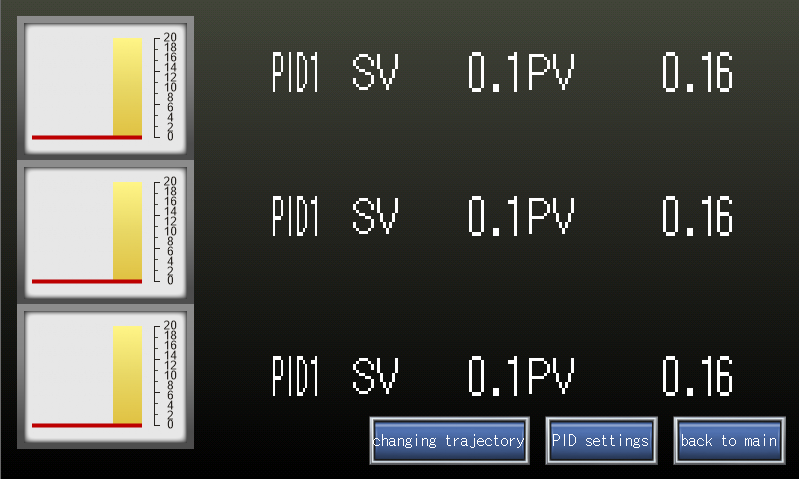
\includegraphics[scale=0.7]{WATER_Main.png}
    \caption{Panel g��wny dla stanowiska Inteco}
    \label{WATER_main}
\end{figure}
\vskip 0.5cm

Ostatnia karta przeznaczona jest to zadawania trajektorii zmian warto�ci zadanej. Jak wspomniano w~poprzednich sekcjach, zaimplementowany zosta� automat stan�w umo�liwiaj�cy zaplanowanie warto�ci zadanych w~trzech r�wnych przedzia�ach czasowych. Jest to mo�liwe poprzez wpisanie odpowiednich warto�ci w~pola widoczne w~prawym g�rnym rogu rys. \ref{WATER_trajectory}. Prze��czenie mi�dzy warto�ciami zadanymi wynikaj�cym z~automatu stanu, a~tymi podanymi na~panelu g��wnym nastepuje na skutek przycisku znajduj�cego si� w~g�rnej cz�ci rysunku. Gdy pod��anie za trajektori� zadan� jest w��czone, aktualny stan automatu wizualizowany jest w~postaci jednej z~lampek zapalanych w~prawym g�rnym rogu ekranu. Okres przedzia��w czasowych konfiguruje si� poprzez zmian� warto�ci pola {\verb duration}.  Wykresy obecne w~lewej cz�ci ekranu oraz przystaj�ce do nich pola liczbowe pozwalaj� monitorowa� poziom rozszczelnienia poszczeg�lnych zawor�w.

\vskip 0.5cm
\begin{figure}[H]
    \centering
    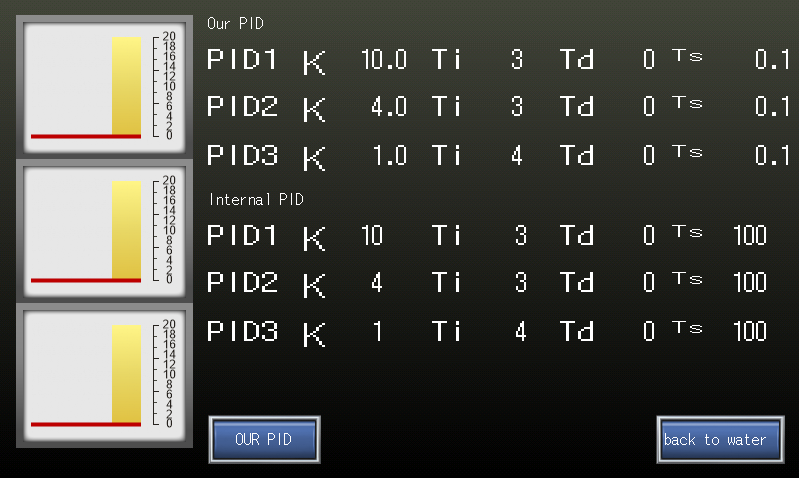
\includegraphics[scale=0.7]{WATER_pid.png}
    \caption{Panel konfiguracyjny regulator�w PID}
    \label{WATER_pid}
\end{figure}
\vskip 0.5cm

\vskip 0.5cm
\begin{figure}[H]
    \centering
    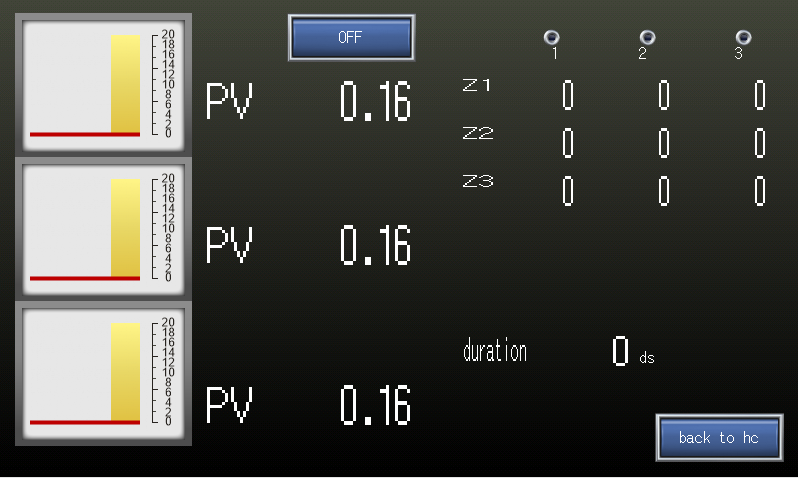
\includegraphics[scale=0.7]{WATER_trajectory.png}
    \caption{Panel konfigurarji trajektorii zadanych.}
    \label{WATER_trajektory}
\end{figure}
\vskip 0.5cm
\chapter{Podsumowanie}

Tak du�y, a~przy tym ostatni projekt z~przedmiotu wymaga pewnej formy podsumowania. Autorska implementacja wielowymiarowych reuglator�w PID oraz DMC s� z~pewno�ci� czym�, co ka�dy student Automatyki i~Robotyki naszego wydzia�u powinien chocia� raz w~�yciu wykona�. Praktyka taka pozwala u�wiadomi� sobie wiele fakt�w niewynikaj�cych wprost z~teorii sterowania, �eby wymeni� chocia� wp�yw braku sprz�enia zwrotnego mi�dzy niezale�nymi regulatorami PID lub praktyczne aspekty wykorzystania modelu w~procesie projektowania uk�adu sterowania. R�wnie� poznanie metod uwzgl�dniania znanych sygna��w zak��ce� w~procesie regulacji jest bardzo korzystnym aspektem wykonanych projekt�w. W~og�lno�ci mo�na powiedzie�, �e koncepcja stoj�ca za projektami realizowanymi w~ramach Projektowania Uk�ad�w Sterowania stanowi dobre podsumowanie wszystkich poprzednich przedmiot�w oscyluj�cych wok� tematu automatyki. Mieli�my przy tej okazji mo�liwo�� powt�rzenia zdobytych do tej pory informacji na temat regulator�w PID oraz DMC, przecie�wiczenia obs�ugi sterownika PLC oraz wykorzystania szerokiego zakresu narz�dzi z~dziedziny identyfikacji i~modelowania poznanych w~toku edukacji. Te aspekty stanowi� mocn� stron� przedmiotu i~w~uznaniu autor�w pozwalaj� okre�li� go mianem obowi�zkowego dla student�w naszego kierunku.

W~ten sps�b kszta�tuj� si� og�lne wnioski wysnute z~perspektywy student�w ko�cz�cych ten przedmiot. Rzeczywisto��, z~kt�r� mierzyli�my si� w~trakcie trwania semestru mia�a jednak odcie� dalece bardziej wpadaj�cy w~czer� rozczarowa�, przygn�bienia i~poczucia marnowanego czasu. Praca automatyka nieodzownie ��czy si� z~potrzeb� akwizycji i~analizy du�ej ilo�ci danych z~obiekt�w regulacji oraz d�ugimi godzinami sp�dzonymi na kalibracji regulator�w, z~czego w~pe�ni zdajemy sobie spraw�. Je�eli jednak do�wiadczenia takie czekaj� nas w~�yciu zawodowym, to czas laboratori�w oraz projekt�w wydaje si� tym bardziej odpowiedni by od takich zagadnie� abstrahowa� w~nieco wi�kszym stopniu, a~uzyskany w~ten spos�b czas przeznaczy� na poszerzenie �wiadomo�ci student�w w~obr�bie omawianej dziedziny.

Ka�dy z~nas s�ysza� o~regulatorach PID czy DMC niejdenokrotnie. Ka�dy niejednokrotnie mia� okazj� je implementowa�. Powtarzanie tych samych informacji na przestrzeni trzech lub czterech przedmiot�w, kt�re przypomnijmy sa obowi�zkowe dla student�we naszego kierunku, wydaje si� by� bezcelowe. Bezcelowo�� takich dzia�a� wydaje si� tym bardziej dosadna je�eli u�wiadomi� sobie, �e poza dwoma wymienionymi regulatorami nie mieli�my okazji zapozna� si� z~innymi podej�ciami do tematu. Poszerzenie wiedzy o~regulacji predykcyjnej poprzez wprowadzenie algorytmu GPC czy ukazanie aspektu stosowalno�ci sztucznych sieci neuronowyh w~sterowaniu to tylko niekt�re z~pomys��w, jakie mog�yby poszerzy� horyzonty student�w, a~przy tym zwi�kszy� ich zaanga�owanie w~przedmiot.

R�wnie� wspomniane ju� godziny sp�dzone na zbieraniu danych z~obiekt�w oraz kolejne godziny przeznaczone na formatowanie ich tak, aby mog�y by� zamieszczone w~obszernych sprawozdaniach realizowanych po ka�dym z~blok�w wydaj� si� w~odczuciach autor�w zb�dne. Zadania takie nie wnosz� niemal nic do zestawu umiej�tno�ci studenta, a~jedynie budz� frustracj� wynikaj�c� z~niemocy zaj�cia si� tematami bardziej warto�ciowymi. W~naszej opinii fakt powtarzania takiego schematu na niemal wszystkich przedmiotach z~omawianej grupy stanowi siln� przes�ank� do podj�cia znacznych zmian w~materii zarz�dzania czasem studenta. Trzymamy kciuki zar�wno za student�w przysz�ych lat jak i~prowadz�cych, aby wsp�ln� prac� wyprwcowali konsensus, kt�ry ��czy�by w~sobie zar�wno dotychczasowy nak�ad pracy wymagany od studenta�w jak i~satysfakcj� wynikaj�c� z~poszerzania przez nich wiedzy i~umiej�tno�ci.

\end{document}
